\chapter{Literature Survey}

\section{Introduction}
In this chapter, we present the results of a literature survey that was performed to identify the current state of obfuscation mechanisms and their impact to the field of code obfuscation.

\subsection{Code Obfuscation and Malware Detectors}

The efficiency of malware detectors against code obfuscation has been a point of discussion
amongst malware researchers for a very long time. A lot of research has been done on the
robustness of malware detectors against high levels of obfuscation ~\cite{Christodorescu}. The issue of malware detector\textquoteright s strengths against obfuscated malware had been discussed as early as 1996, as can be
seen in the quote by S.Gordon and R.Ford ~\cite{gordon}: \\
\textquoteleft The evaluation of anti-virus software is not adequately covered by any existing criteria based
on formal methods. The process, therefore, has been carried out by various personnel using a
variety of tools and methods.\textquoteright


\subsection{Program Obfuscation}

There has been a lot of theoretical research on the different aspects of obfuscation and on ways to improve it. Most of this research has been successful in arriving at a conclusion on the efficiency of the cryptographic problems of encryption, authentication and protocol ~\cite{barak}. But the problem of program obfuscation has remained an area within cryptography in which theoretical research has been inadequate. In their seminal paper on program obfuscation, Barak et al. ~\cite{barak} propose to represent program obfuscation as below:
An obfuscator O is said to be an efficient compiler if it takes as input a program P and produces a program O(P) and satisfies the following two conditions:
\begin{enumerate}
	\item Functionality: O(P) computes the same function as P
	\item \textquoteleft Virtual Black Box\textquoteright property: Anything that can be efficiently computed from O(P) can also be computed by P.
\end{enumerate}

The paper by Christodorescu et al. ~\cite{Christodorescu} lists various ways to test and achieve program obfuscation in general. A detailed analysis of the various obfuscation methods is also discussed in the paper. One interesting angle explored by the paper deals with assigning mathematical equations to measure the effectiveness of the individual obfuscators. This lets us quantify the different obfuscators and rank them against each other.
One of the evasion methods employed in malware obfuscation is polymorphism. It is a method by which a program evades various detection tools by mutating into different forms. In the paper by Rastogi et al.~\cite{rastogi}, the authors develop and propose a framework called \textquoteleft DroidChameleon \textquoteright that provides a way to transform Android applications into different forms with minimal user involvement. 

\begin{figure}[htb]
	\centering
	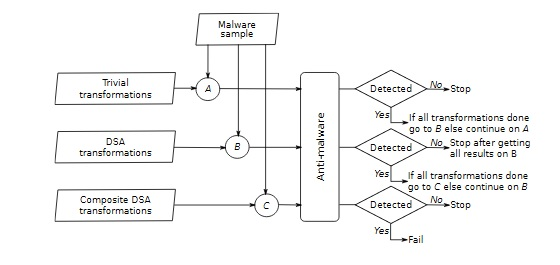
\includegraphics[width=0.5\textwidth]{evalFigure1.jpg}
	\caption{Evaluating anti-malware} 
	\label{fig:eval}
\end{figure}

As shown in Fig. ~\ref{fig:eval}, the authors apply various transformations on a malware sample dataset. The output of all these transformations are processed by a malware detector (referred here as Anti-malware).  The input to the anti-malware is processed sequentially. After each transformation, the anti-malware’s output is evaluated and if the malware detection fails, the next level of transformation is applied. This helps rank the various malware detectors against each other for accurate analysis.

\section{OBFUSCATION IN ANDROID MALWARE}

A report by Google stated that a majority of malware detectors work as a binary classifier~\cite{google}. They classify an application as a malware or a benign file. In order to effectively eliminate malicious applications, it is important that malware detectors do more than just identify malware. They should be able to isolate the core parts of the application that perform the malicious acts and work at fixing the loopholes that let the program act in a malicious way. More recent malware applications employ a variety of tricks, in addition to traditional code obfuscation mechanisms. For instance, a variant of Android malware, known as Android/BadAccent, is a known banking Trojan, that steals credentials used in banking applications~\cite{rasthofer2015}. A variant of this malware used a mechanism known as “Tapjacking” to extract the credentials from the users. In this form of attack, a screen is displayed to the user, while a second screen is hidden behind the actual visible display ~\cite{chen2014peeking}. When a user clicks a button on the screen, assuming it to be the one that is displayed, the underlying screen gathers the input and processes the command.  This is a common method of gathering details from unsuspecting users.


\subsection{STATISTICAL ANALYSIS TECHNIQUES AND ANDROID MALWARE}

One widely used approach for analyzing malware samples is the usage of statistical methods. In such methods, the Android executable file (with the extension apk), is decompiled to get the original source code. Due to the Android operating system being written in Java, it is easy to reverse engineer an apk file to retrieve the source code. This opens up many opportunities for performing statistical analysis on the obtained raw data. This also lets a researcher perform various operations on the source code, and then repackage it back into an apk. In the approach known as AndroSimilar, Faruki et al. ~\cite{androsimilar} propose a new algorithm that takes into consideration various features that are known to be present in malware alone. The AndroSimiar approach, as shown in Fig.~\ref{fig:andro} decompiles an apk file and repackages it after feature extraction. To extract the features, the algorithm incorporates apps from the Google Playstore and other third party applications. These features are normalized and fed into a signature generation engine, that provides a unique signature for each malware. This is used as reference for detecting future malware applications.


\begin{figure}[htb]
	\centering
	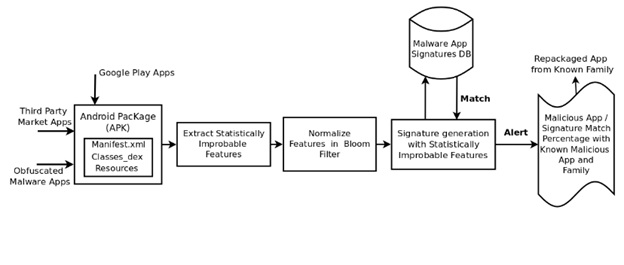
\includegraphics[width=0.5\textwidth]{androSimilar.jpg}
	\caption{AndroSimilar} 
	\label{fig:andro}
\end{figure}

\section{Conclusion}

Malware in mobile devices is no longer a problem confined to labs and research areas. The rapid increase in access to computers has helped malware writers create specific, targeted programs that perform with high efficiency and exploit vulnerabilities in different operating systems. The amount of research being done in malware analysis and, more specifically, in Android malware, is in the right direction. In the fight against sophisticated metamorphic malware, it is imperative that the malware detector is better than the malware creator. In this paper, we have explored various work, that dealt with the different aspects of malware obfuscation and ways to overcome the shortcomings in today\textquoteright s version of malware detectors. The future of malware looks very bright and it is hoped that the malware detectors of the future will be up to the task at hand.

